\documentclass[border=2pt]{standalone}
% Computer Modern, the font of the handouts (pdflatex)
\usepackage{amsmath}
\usepackage{tikz}
\usepackage{pgfplots}
\pgfplotsset{compat=1.18}
\usetikzlibrary{arrows.meta,calc}
\definecolor{cA}{HTML}{2A78D6}
\definecolor{cB}{HTML}{EB6834}
\definecolor{cC}{HTML}{1BAF7A}
\definecolor{cD}{HTML}{EDA100}
\definecolor{cE}{HTML}{E87BA4}
\definecolor{nodeblue}{HTML}{1565C0}
\definecolor{linkgray}{HTML}{546E7A}
\definecolor{lightgray}{HTML}{CFD8DC}
\definecolor{txt}{HTML}{263238}
\definecolor{band}{HTML}{EEEEEE}
\definecolor{uUnused}{HTML}{BDBDBD}
\definecolor{uLow}{HTML}{2E7D32}
\definecolor{uMid}{HTML}{F9A825}
\definecolor{uHigh}{HTML}{EF6C00}
\definecolor{uFull}{HTML}{C62828}
\definecolor{uOver}{HTML}{7B1FA2}
\tikzset{
  nd/.style={circle, fill=nodeblue, draw=white, line width=0.7pt, minimum size=#1, inner sep=0pt},
  nd/.default=3.2mm,
  nlab/.style={font=\footnotesize\bfseries, text=txt, inner sep=1pt},
  lbl/.style={font=\scriptsize, text=txt, fill=white, fill opacity=0.85, text opacity=1, inner sep=0.7pt},
  arr/.style={-{Stealth[length=1.9mm, width=1.5mm]}},
}
\pgfplotsset{
  lab/.style={
    scale only axis, axis lines*=left, grid=major, grid style={black!12},
    tick label style={font=\small}, label style={font=\normalsize},
    ylabel style={align=center},
    legend style={draw=none, fill=none, font=\small},
    legend cell align=left, tick align=outside, axis line style={black!60},
    every axis plot/.append style={line width=1.1pt},
  },
  % the series differ in color, marker and line style (readable in black and white);
  % the second series has hollow markers, visible where the two curves overlap
  s1/.style={cA, solid, mark=*, mark size=1.7pt},
  s2/.style={cB, densely dashed, mark=square*, mark size=1.6pt, mark options={solid, fill=white}},
  s3/.style={cC, dashdotted, mark=diamond*, mark size=2.1pt, mark options={solid}},
  s4/.style={cD, densely dotted, mark=triangle*, mark size=2.1pt, mark options={solid, fill=white}},
  s5/.style={cE, dashed, mark=triangle*, mark size=2.1pt, mark options={solid, rotate=180}},
  ebars/.style={error bars/.cd, y dir=both, y explicit,
    error bar style={solid, line width=0.9pt}, error mark options={solid, rotate=90, mark size=2.2pt}},
}
\begin{document}
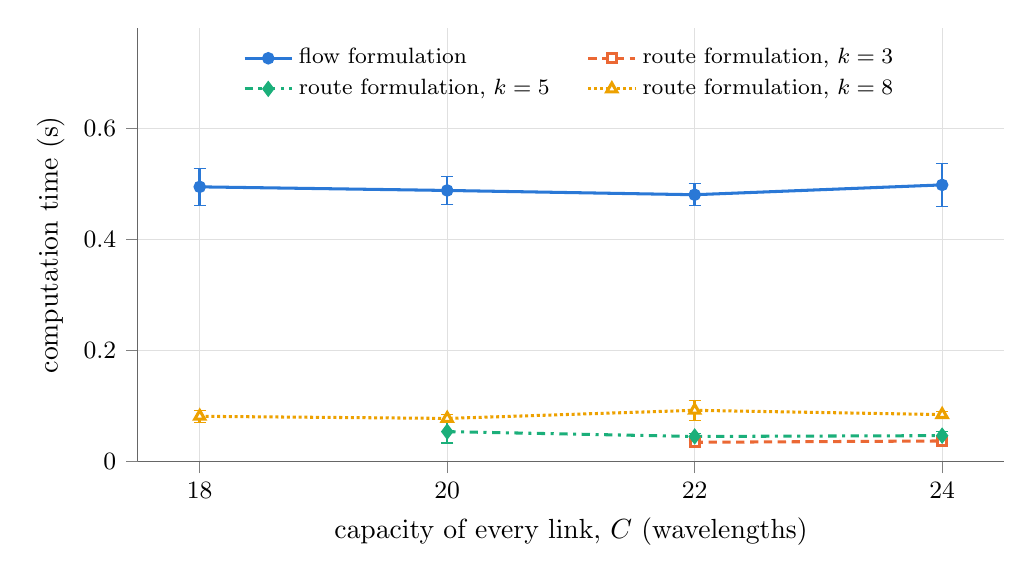
\begin{tikzpicture}\begin{axis}[lab, width=110mm, height=55mm, xmin=17.5, xmax=24.5, ymin=0, ymax=0.78, xtick=data, ytick distance=0.2, xlabel={capacity of every link, $C$ (wavelengths)}, ylabel={computation time (s)}, legend columns=2, legend style={font=\footnotesize, at={(0.5,0.98)}, anchor=north, /tikz/every even column/.append style={column sep=4mm}}]
\addplot[s1, ebars] coordinates {(18,0.4943) +- (0,0.0331) (20,0.4878) +- (0,0.0249) (22,0.4801) +- (0,0.0199) (24,0.4978) +- (0,0.0382)};
\addlegendentry{flow formulation}
\addplot[s2, ebars] coordinates {(22,0.0342) +- (0,0.0023) (24,0.0366) +- (0,0.0054)};
\addlegendentry{route formulation, $k = 3$}
\addplot[s3, ebars] coordinates {(20,0.0534) +- (0,0.0204) (22,0.0447) +- (0,0.0048) (24,0.0462) +- (0,0.0071)};
\addlegendentry{route formulation, $k = 5$}
\addplot[s4, ebars] coordinates {(18,0.0810) +- (0,0.0106) (20,0.0772) +- (0,0.0070) (22,0.0918) +- (0,0.0179) (24,0.0841) +- (0,0.0056)};
\addlegendentry{route formulation, $k = 8$}
\end{axis}\end{tikzpicture}
\end{document}
